\clearpage
\section{Statistics: from means to distributions and null models}
\label{sec:statistics}
% EDITORIAL ADDITION: navigation or conceptual bridge
A mean can conceal variation between cells, molecules, or populations.
Probability distributions specify that variation; a master equation specifies how the distribution changes.
The mRNA example links this chapter directly to the deterministic model in section~\ref{sec:mrna-mean}.
% Source: day3.tex:1121; unit d3.8.0
\subsection{Probability and quantitative null hypotheses}
\label{sec:null}


% ============================================================

A useful null hypothesis is the simplest random process that could plausibly generate the observations.
The purpose of the null hypothesis is to ask what behavior we should expect even without invoking an additional mechanism.
Probability distributions provide mathematical descriptions of the fluctuations expected under different random processes.

% ------------------------------------------------------------

% EDITORIAL ADDITION: navigation or conceptual bridge
For a discrete random variable, probabilities sum to one and expectations are probability-weighted sums.
For a continuous variable, a probability density integrates to one and expectations are integrals.
Appendix~\ref{math:probability} summarizes normalization, expectation, and variance.
% Source: day3.tex:1187; unit d3.8.2
\subsection{Recurring probability distributions}
\label{sec:distributions}

% ============================================================

Different stochastic processes naturally give rise to different probability distributions.
For a discrete variable, probabilities are specified by a probability mass function (PMF).
For a continuous variable, they are specified by a probability density function (PDF), whose integral over an interval gives the probability of that interval.

Some recurring distributions in physical biology are (see Table~\ref{tab: prob_distributions}):
\begin{enumerate}
    \item binomial
    \item Poisson
    \item Gaussian
    \item exponential
    \item geometric
\end{enumerate}


\begin{table}[h]
\centering
\footnotesize
\renewcommand{\arraystretch}{1.18}

\begin{tabularx}{\textwidth}{
    |>{\raggedright\arraybackslash}p{2.5cm}
    |>{\raggedright\arraybackslash}p{5.5cm}
    |>{\centering\arraybackslash}p{1cm}
    |>{\centering\arraybackslash}p{1.6cm}
    |>{\raggedright\arraybackslash}X|
}
\hline
\textbf{Distribution} &
\textbf{PMF/PDF} &
\textbf{Mean} &
\textbf{Variance} &
\textbf{Representative examples}
\\
\hline
Binomial \newline \newline \miniBinomial & 
$\displaystyle P(k)=\binom{n}{k}p^k(1-p)^{n-k}$ &
$np$ &
$np(1-p)$ &
Receptor occupancy among $n$ independent receptors; rightward steps in an $n$-step random walk; protein partitioning at cell division.
\\
\hline
Poisson \newline \newline \miniPoisson & 
$\displaystyle P(k)=e^{-\lambda}\frac{\lambda^k}{k!}$ &
$\lambda$ &
$\lambda$ &
Mutations per genome; deaths from horse kicks per army corps; wartime bomb hits per district; photons detected during a fixed time interval.
\\
\hline
Gaussian \newline \newline \miniGaussian & 
$\displaystyle p(x)=\frac{1}{\sqrt{2\pi\sigma^2}}\exp\left[-\frac{(x-\mu)^2}{2\sigma^2}\right]$ &
$\mu$ &
$\sigma^2$ &
Errors in repeated measurements; displacement after many diffusive steps; polymer end-to-end displacement; variation in human height.
\\
\hline
Exponential \newline \newline \miniExponential &
$\displaystyle p(t)=\lambda e^{-\lambda t}$ &
$\displaystyle \frac{1}{\lambda}$ &
$\displaystyle \frac{1}{\lambda^2}$ &
Waiting time until radioactive decay; time between constant-rate events; lifetime of a molecular state; waiting time until the next photon.
\\
\hline
Geometric \newline \newline \miniGeometric &
$\displaystyle P(n)=(1-p)^n p$ &
$\displaystyle \frac{1-p}{p}$ &
$\displaystyle \frac{1-p}{p^2}$ &
Failures before the first success; unsuccessful chromosome-capture attempts; tails before the first head; rejected proofreading attempts.
\\
\hline
\end{tabularx}

\caption{Common probability distributions and representative examples.
The geometric distribution is defined here as the number of failures before the first success.}
\label{tab: prob_distributions}
\end{table}

% The distributions describe different kinds of random variables and different underlying stochastic processes.
% The binomial distribution describes the number of successes in a fixed number of independent trials.
% The Poisson distribution describes the number of events occurring when independent events happen at a constant average rate.
% The Gaussian distribution commonly arises when a quantity is the sum of many independent contributions.
% The exponential distribution describes the waiting time until the next event in a constant-rate process.
% The geometric distribution is the discrete analogue of the exponential distribution and describes how many independent trials occur before the first success.


% EDITORIAL CHANGE: replace chronological phrasing
The binomial, Poisson, and Gaussian distributions recur throughout the course examples.
The exponential distribution describes an important new class of problems: waiting times.

% ------------------------------------------------------------

% Source: day3.tex:1204; unit d3.8.3
\subsubsection{Waiting times and molecular binding}
\label{sec:waiting}

% ------------------------------------------------------------

The exponential distribution describes the waiting time until an event occurs when that event happens with a constant rate.
Let the event occur at rate $\lambda$.
The probability density for the waiting time $t$ is
\[
    \boxed{p(t)=\lambda e^{-\lambda t}, \qquad t\geq0.}
\]
The mean waiting time is
\[
    \langle t\rangle = \frac{1}{\lambda},
\]
and the variance is
\[
    \operatorname{Var}(t)=\frac{1}{\lambda^2}.
\]

\paragraph{Example: molecular binding times}

Single-molecule fluorescence experiments can resolve individual association and dissociation events.
For example, Wang et al.\ immobilized fluorescently labelled DNA molecules on a surface and observed the binding of fluorescently labelled $\lambda$ repressor proteins \cite{wang2009quantitative}.
When a protein was bound to a DNA molecule, the two fluorescence signals were observed at the same location.
The resulting signal could be represented by a two-state time trace,
\[
    I(t)=
    \begin{cases}
        1, & \text{protein bound},\\
        0, & \text{protein unbound}.
    \end{cases}
\]
A sequence of binding and unbinding events then appears as alternating intervals in which $I(t)=1$ and $I(t)=0$.
% 
\paragraph{Bound-state lifetime}
Suppose a bound protein dissociates with a constant rate $k_{\mathrm{off}}$.
Let $S(t)$ be the probability that a protein which was bound at time $t=0$ is still bound after time $t$.
During a small interval $\Delta t$, the probability of dissociation is
% 
\[
    k_{\mathrm{off}}\Delta t.
\]
% 
The probability of remaining bound is therefore
% 
\[
    1-k_{\mathrm{off}}\Delta t.
\]
% 
The update rule is
% 
\[
    S(t+\Delta t)=S(t)\left(1-k_{\mathrm{off}}\Delta t\right).
\]
% 
Taking the continuous-time limit gives
% 
\[
    \frac{\dd S}{\dd t}=-k_{\mathrm{off}}S.
\]
% 
With the initial condition $S(0)=1$,
% 
\[
    \boxed{S(t)=e^{-k_{\mathrm{off}}t}.}
\]
% 
This is the probability that the protein remains bound for at least time $t$.
The probability density for the actual bound lifetime $t_{\mathrm{on}}$ is obtained from
% 
\[
    p(t_{\mathrm{on}})=-\frac{\dd S}{\dd t_{\mathrm{on}}}.
\]
% 
Therefore,
% 
\[
    \boxed{ p(t_{\mathrm{on}})=k_{\mathrm{off}}e^{-k_{\mathrm{off}}t_{\mathrm{on}}}. }
\]
% 
The mean bound lifetime is
% 
\[
    \langle t_{\mathrm{on}}\rangle = \frac{1}{k_{\mathrm{off}}}.
\]
% 
Thus measuring the distribution of bound-state durations provides a way to estimate the dissociation rate $k_{\mathrm{off}}$.
% 
\paragraph{Waiting for binding}
The unbound intervals can be treated similarly.
If binding occurs with an effective constant rate $\lambda_{\mathrm{on}}$, then
% 
\[
    p(t_{\mathrm{off}})=\lambda_{\mathrm{on}}e^{-\lambda_{\mathrm{on}}t_{\mathrm{off}}}.
\]
% 
If $k_{\mathrm{on}}$ is a bimolecular association rate constant and the protein concentration is $[P]$, then the effective rate is
% 
\[
    \lambda_{\mathrm{on}}=k_{\mathrm{on}}[P].
\]
% 
The important distinction is therefore
% 
\[
    \text{bound lifetime} \longleftrightarrow k_{\mathrm{off}},
\]
% 
whereas
% 
\[
    \text{unbound waiting time} \longleftrightarrow k_{\mathrm{on}}[P].
\]

% ------------------------------------------------------------

% Source: day3.tex:1329; unit d3.8.4
% \subsubsection{Distribution reference table}
% \label{sec:dist-table}

% ------------------------------------------------------------


% Source: day2.tex:282; unit d2.3
\subsection{The theory of the histogram}
\label{sec:histogram}


% ============================================================

The theory of the mean follows only the average value of a variable.
In many biological systems, however, the full distribution contains information that the mean alone cannot capture.
Instead of asking only how the mean changes with time, we can ask how probability moves between different possible values or states.

% ------------------------------------------------------------
\subsubsection*{Example 1: number of mRNA molecules in a fly embryo}
% ------------------------------------------------------------

Suppose we want to describe the spatial distribution of mRNA molecules along a fly embryo.
We can discretize the embryo into small spatial boxes.
Each box then contains some number of mRNA molecules.
The collection of counts across boxes forms a spatial distribution rather than a single mean value.


% ------------------------------------------------------------
\subsubsection*{Example 2: age distributions}
% ------------------------------------------------------------

Age is intrinsically continuous, but it can be discretized into bins such as years.
For example,
\[
    [0,1), \qquad [1,2), \qquad [2,3), \qquad \ldots
\]
We can then count how many individuals occupy each age bin.
The resulting histogram is a discretized representation of the underlying age distribution.


% ============================================================
\subsubsection{Theory of the histogram protocol}
% ============================================================

A corresponding protocol for describing an entire probability distribution is:

\begin{enumerate}
    \item Consider the population of interest as a probability distribution over a set of possible states or bins.
    \item Enumerate all the ways in which individuals or probability can move between those bins.
    \item Write an update rule describing the flow of probability into and out of each bin during a time step $\Delta t$.
    \item Given an initial distribution $p(m,t_0)$, solve for the distribution $p(m,t)$ at later times.
\end{enumerate}

Here $m$ labels the state or bin of interest.
For example, $m$ could denote the number of mRNA molecules in a cell.

Instead of following only the mean
$\langle m\rangle$,
we now follow the full probability distribution
\[
    p(m,t).
\]
The normalization condition is
\[
    \sum_m p(m,t)=1.
\]
This shift from the dynamics of a mean to the dynamics of a distribution is important whenever fluctuations are themselves biologically relevant.

% ------------------------------------------------------------
\subsubsection{Example: the dynamics of an mRNA histogram}
% ------------------------------------------------------------

Consider a population of identical cells.
Instead of describing only the mean number of mRNA molecules per cell, we describe the entire distribution of mRNA copy numbers.

Let
\[
    p(m,t)
\]
denote the probability that a cell contains exactly $m$ mRNA molecules at time $t$.
Equivalently, if we measure a large population of cells, $p(m,t)$ is the fraction of cells occupying the histogram bin corresponding to $m$ mRNAs.

The distribution is normalized,
\[
    \sum_{m=0}^{\infty}p(m,t)=1.
\]
% % % 
% % % 
% ------------------------------------------------------------
\paragraph{Step 1: identify the states}
% ------------------------------------------------------------
The possible states are the discrete mRNA copy numbers
\[
    m=0,1,2,3,\ldots
\]
Each value of $m$ corresponds to one bin of the histogram.
% % 
% % 
% ------------------------------------------------------------
\paragraph{Step 2: enumerate the ways of moving between bins}
% ------------------------------------------------------------
Assume that mRNA is produced at a constant rate $r$.
% 
A transcription event increases the copy number by one,
% 
\[
    m \longrightarrow m+1.
\]
% 
Assume that each individual mRNA molecule is degraded independently at rate $\gamma$.
% 
If there are $m$ molecules in the cell, the total degradation rate is therefore
% 
\[
    \gamma m.
\]
% 
A degradation event decreases the copy number by one,
% 
\[
    m \longrightarrow m-1.
\]
% 
The transitions between neighboring histogram bins are therefore
% 
\[
    \cdots \rightleftharpoons m-1 \rightleftharpoons m \rightleftharpoons m+1 \rightleftharpoons \cdots
\]
% 
with transcription moving probability to the right and degradation moving probability to the left.
\\
% 
% 
% ------------------------------------------------------------
\paragraph{Step 3: write the probability flow for one bin}
% ------------------------------------------------------------
To determine how $p(m,t)$ changes, enumerate all the ways probability can flow into and out of the bin $m$ during a short time interval $\Delta t$.
There are two ways to enter the state $m$.
First, a cell containing $m-1$ molecules can produce one new mRNA.
The corresponding probability flow is
\[
    r\Delta t\,p(m-1,t).
\]
Second, a cell containing $m+1$ molecules can lose one mRNA through degradation.
Since there are $m+1$ molecules available to degrade, the total degradation rate in this state is $\gamma(m+1)$.
The corresponding probability flow is
\[
    \gamma(m+1)\Delta t\,p(m+1,t).
\]

There are also two ways to leave the state $m$.
A transcription event moves the system from $m$ to $m+1$, giving an outgoing contribution
\[
    r\Delta t\,p(m,t).
\]
A degradation event moves the system from $m$ to $m-1$, giving an outgoing contribution
\[
    \gamma m\Delta t\,p(m,t).
\]
Putting all of these contributions together gives the update rule
\[
    \begin{aligned}
        p(m,t+\Delta t)={}&p(m,t)+r\Delta t\,p(m-1,t)+\gamma(m+1)\Delta t\,p(m+1,t)
        \\
        &{}-r\Delta t\,p(m,t)-\gamma m\Delta t\,p(m,t).
    \end{aligned}
\]
Its structure is simply
\[
    \text{new probability}=\text{old probability}+\text{flowing in}-\text{flowing out}.
\]
% 
% 
% ------------------------------------------------------------
\paragraph{Step 4: take the continuous-time limit}
% ------------------------------------------------------------
Subtracting $p(m,t)$ from both sides and dividing by $\Delta t$ gives
% 
\[
    \begin{aligned}
        \frac{p(m,t+\Delta t)-p(m,t)}{\Delta t}={}&rp(m-1,t)+\gamma(m+1)p(m+1,t)
        \\
        &{}-rp(m,t)-\gamma m p(m,t).
    \end{aligned}
\]
% 
Taking the limit $\Delta t\rightarrow0$ gives
% 
\begin{equation}
    \boxed{ \frac{\partial p(m,t)}{\partial t} = rp(m-1,t) + \gamma(m+1)p(m+1,t) - rp(m,t) - \gamma m p(m,t) }.
    \label{eq:mrna-master}
\end{equation}
% 
This is the chemical master equation for constitutive mRNA production and degradation.
It describes the dynamics of the entire histogram rather than only the mean mRNA number.
% 
% 
% ------------------------------------------------------------
\paragraph{Reading the master equation as probability flow}
% ------------------------------------------------------------
Each term has a direct interpretation:
\begin{enumerate}
    \item $rp(m-1,t)$ : probability flowing into bin $m$ from bin $m-1$ through transcription.
    \item $\gamma(m+1)p(m+1,t)$ : probability flowing into bin $m$ from bin $m+1$ through degradation.
    \item $-rp(m,t)$ : probability leaving bin $m$ through transcription.
    \item $-\gamma m p(m,t)$ : probability leaving bin $m$ through degradation.
\end{enumerate}
Therefore the equation is simply a bookkeeping equation for probability.
% 
% 
% ------------------------------------------------------------
\paragraph{Boundary at zero mRNAs}
% ------------------------------------------------------------
The copy number cannot become negative.
For $m=0$, there is therefore no probability flow into the state from $m=-1$.
The equation for the zero-mRNA bin is
\[
    \frac{\partial p(0,t)}{\partial t} = \gamma p(1,t) - rp(0,t).
\]
The first term represents cells entering the $m=0$ state when their last mRNA is degraded.
The second term represents cells leaving the $m=0$ state when a new mRNA is produced.
% 
% 
% ------------------------------------------------------------
\paragraph{Steady-state histogram}
% ------------------------------------------------------------
At steady state, the probability of occupying each bin no longer changes with time,
\[
    \frac{\partial p(m,t)}{\partial t}=0.
\]
For this simple birth--death process, the steady-state distribution is a Poisson distribution,
\[
    p_{\mathrm{ss}}(m) = \frac{\lambda^m e^{-\lambda}}{m!},
\]
where the parameter $\lambda = \frac{r}{\gamma}$.
Therefore,
\[
    \boxed{ p_{\mathrm{ss}}(m) = \frac{1}{m!} \left(\frac{r}{\gamma}\right)^m e^{-r/\gamma} }.
\]
The mean of this distribution is
\[
    \langle m\rangle_{\mathrm{ss}}=\frac{r}{\gamma}.
\]
Its variance is also
\[
    \operatorname{Var}(m)_{\mathrm{ss}}=\frac{r}{\gamma}.
\]
% 
% 
% ------------------------------------------------------------
\paragraph{Connection to the theory of the mean}
% ------------------------------------------------------------
The histogram description contains the mean description as one of its consequences.
The mean mRNA number is defined from the probability distribution as
\[
    \langle m(t)\rangle = \sum_{m=0}^{\infty}m\,p(m,t).
\]
Taking the mean of the master equation~\eqref{eq:mrna-master} gives
\[
    \boxed{ \frac{\dd\langle m\rangle}{\dd t} = r-\gamma\langle m\rangle }.
\]
This is exactly the deterministic mean equation~\eqref{eq:mrna-mean}.
At steady state,
\[
    \langle m\rangle_{\mathrm{ss}}=\frac{r}{\gamma}.
\]

The two approaches therefore answer different levels of the same question.
The theory of the mean tells us how the average copy number evolves.
The theory of the histogram tells us how the probability of every possible copy number evolves.
The histogram description consequently contains information about fluctuations, variance, and the shape of the population distribution that is invisible if we follow only the mean.
% 

% ------------------------------------------------------------
The simple mRNA birth--death model assumes that:

\begin{itemize}
    \item transcription occurs at a constant rate $r$ independent of the current mRNA number;
    \item each mRNA molecule degrades independently at the same rate $\gamma$;
    \item transcription changes the copy number by exactly $+1$;
    \item degradation changes the copy number by exactly $-1$;
    \item the system is Markovian, so transition probabilities depend only on the current state;
    \item $\Delta t$ is sufficiently small that the probability of two or more reaction events during the same time interval is of order $\Delta t^2$ and can be neglected;
    \item there is no transcriptional bursting, promoter switching, feedback, or other regulation;
    \item cells are treated as identical apart from the stochastic differences generated by transcription and degradation.
\end{itemize}
These assumptions define a deliberately simple null model rather than a universal description of transcription.
Single-cell measurements show that real transcription can involve promoter switching and burst-like production, producing fluctuations not captured by the constitutive birth-death model \cite{golding2005real}.

% ============================================================

% EDITORIAL ADDITION: navigation or conceptual bridge
A spatial profile across embryo positions and a copy-number histogram across cells use different bins.
In the first case, the bin labels a position; in the second, it labels a molecular count.
The update protocol must specify both the state variable and the population being represented.
% Source: day3.tex:1129; unit d3.8.1
\subsection{Case study: the Buri experiment and genetic drift}
\label{sec:buri}

% ------------------------------------------------------------

Peter Buri's experiment provides a classic demonstration of genetic drift in small populations.
Buri studied many independent populations of \textit{Drosophila melanogaster}.
In one experimental series, 107 replicate populations were followed for 19 generations.
Each population was initiated with 16 heterozygous flies.
At every subsequent generation, 8 males and 8 females were randomly selected from the offspring to found the next generation.
The population size was therefore kept small, while the particular alleles passed to the next generation were determined partly by random sampling (Fig.~\ref{fig:buri-drift}) \cite{buri1956gene}.
%
% 
\paragraph{Allele frequency}
Using the red, orange, and white notation from the lecture, suppose that red flies carry two copies of the red allele, orange flies are heterozygous, and white flies carry no copies of the red allele.
If there are $N_{\mathrm{red}}$ red flies, $N_{\mathrm{orange}}$ orange flies, and $N_{\mathrm{flies}}$ flies in total, then the frequency of the red allele is
\[
    p_{\mathrm{red}} = q(bw^{75}) = \frac{2N_{\mathrm{red}}+N_{\mathrm{orange}}}{2N_{\mathrm{flies}}}.
\]

The factor of two in the denominator appears because each diploid fly carries two copies of the locus.
Initially, all 16 flies are heterozygous, so
\[
    p_{\mathrm{red}} = \frac{16}{32} = \frac{1}{2}.
\]

As an example, suppose a later generation contains 4 red, 2 white, and 10 orange flies.
Then
\[
    p_{\mathrm{red}} = \frac{2(4)+10}{2(16)} = \frac{18}{32} = 0.5625.
\]
% 
\paragraph{Genetic drift}
Even when the two alleles have the same fitness, random sampling means that their frequencies do not remain exactly constant from one generation to the next.
One population may contain slightly more copies of the red allele, while another may contain slightly fewer.
These small fluctuations accumulate over generations.
Different replicate populations therefore wander away from the common initial allele frequency,
\[
    p_{\mathrm{red}}=\frac{1}{2}.
\]
Eventually, some populations reach
\[
    p_{\mathrm{red}}=1,
\]
meaning that the red allele has become fixed.
Others reach
\[
    p_{\mathrm{red}}=0,
\]
meaning that the red allele has been lost and the alternative allele has become fixed.
These states are absorbing: once an allele has disappeared from a closed population, random sampling alone cannot bring it back.
Thus substantial differences between populations can arise from random sampling alone, without invoking a selective advantage.
This random change in allele frequency is called \emph{genetic drift}.

% ============================================================

% Source: day5.tex:78; unit d5.1.2
\label{sec:buri-vector}
Each vial contains 16 diploid flies, so there are
\[
    2\times16=32
\]
copies of the relevant locus.

Let $n_R$ denote the number of red alleles in a vial.
The possible values are
\[
    n_R=0,1,2,\ldots,32.
\]
There are therefore 33 possible allele-count states.

The allele count $n_R$ itself is a single discrete variable.
However, a probability distribution over all possible allele counts can be represented by a vector with 33 components,
\[
    \mathbf{p} =
    \begin{pmatrix}
        p_0 \\
        p_1 \\
        \vdots \\
        p_{32}
    \end{pmatrix}.
\]
Here
\[
    p_i=P(n_R=i).
\]
The vector therefore lives in a 33-dimensional vector space, although not every vector in that space is a valid probability distribution.
The components must satisfy
\[
    p_i\geq0
\]
and
\[
    \sum_{i=0}^{32}p_i=1.
\]
Thus a stochastic evolutionary process can be viewed as the time evolution of a probability vector over the possible allele-count states.


% ============================================================

% EDITORIAL ADDITION: navigation or conceptual bridge
The 33-component representation describes the distribution over allele counts.
It is useful even when the distribution mean does not reveal how populations accumulate at the absorbing states.
Section~\ref{sec:vectors} extends the vector idea to other biological data.


\begin{figure}[h]
    \centering

    \begin{minipage}[t]{0.31\textwidth}
        \vspace{0pt}
        \centering
        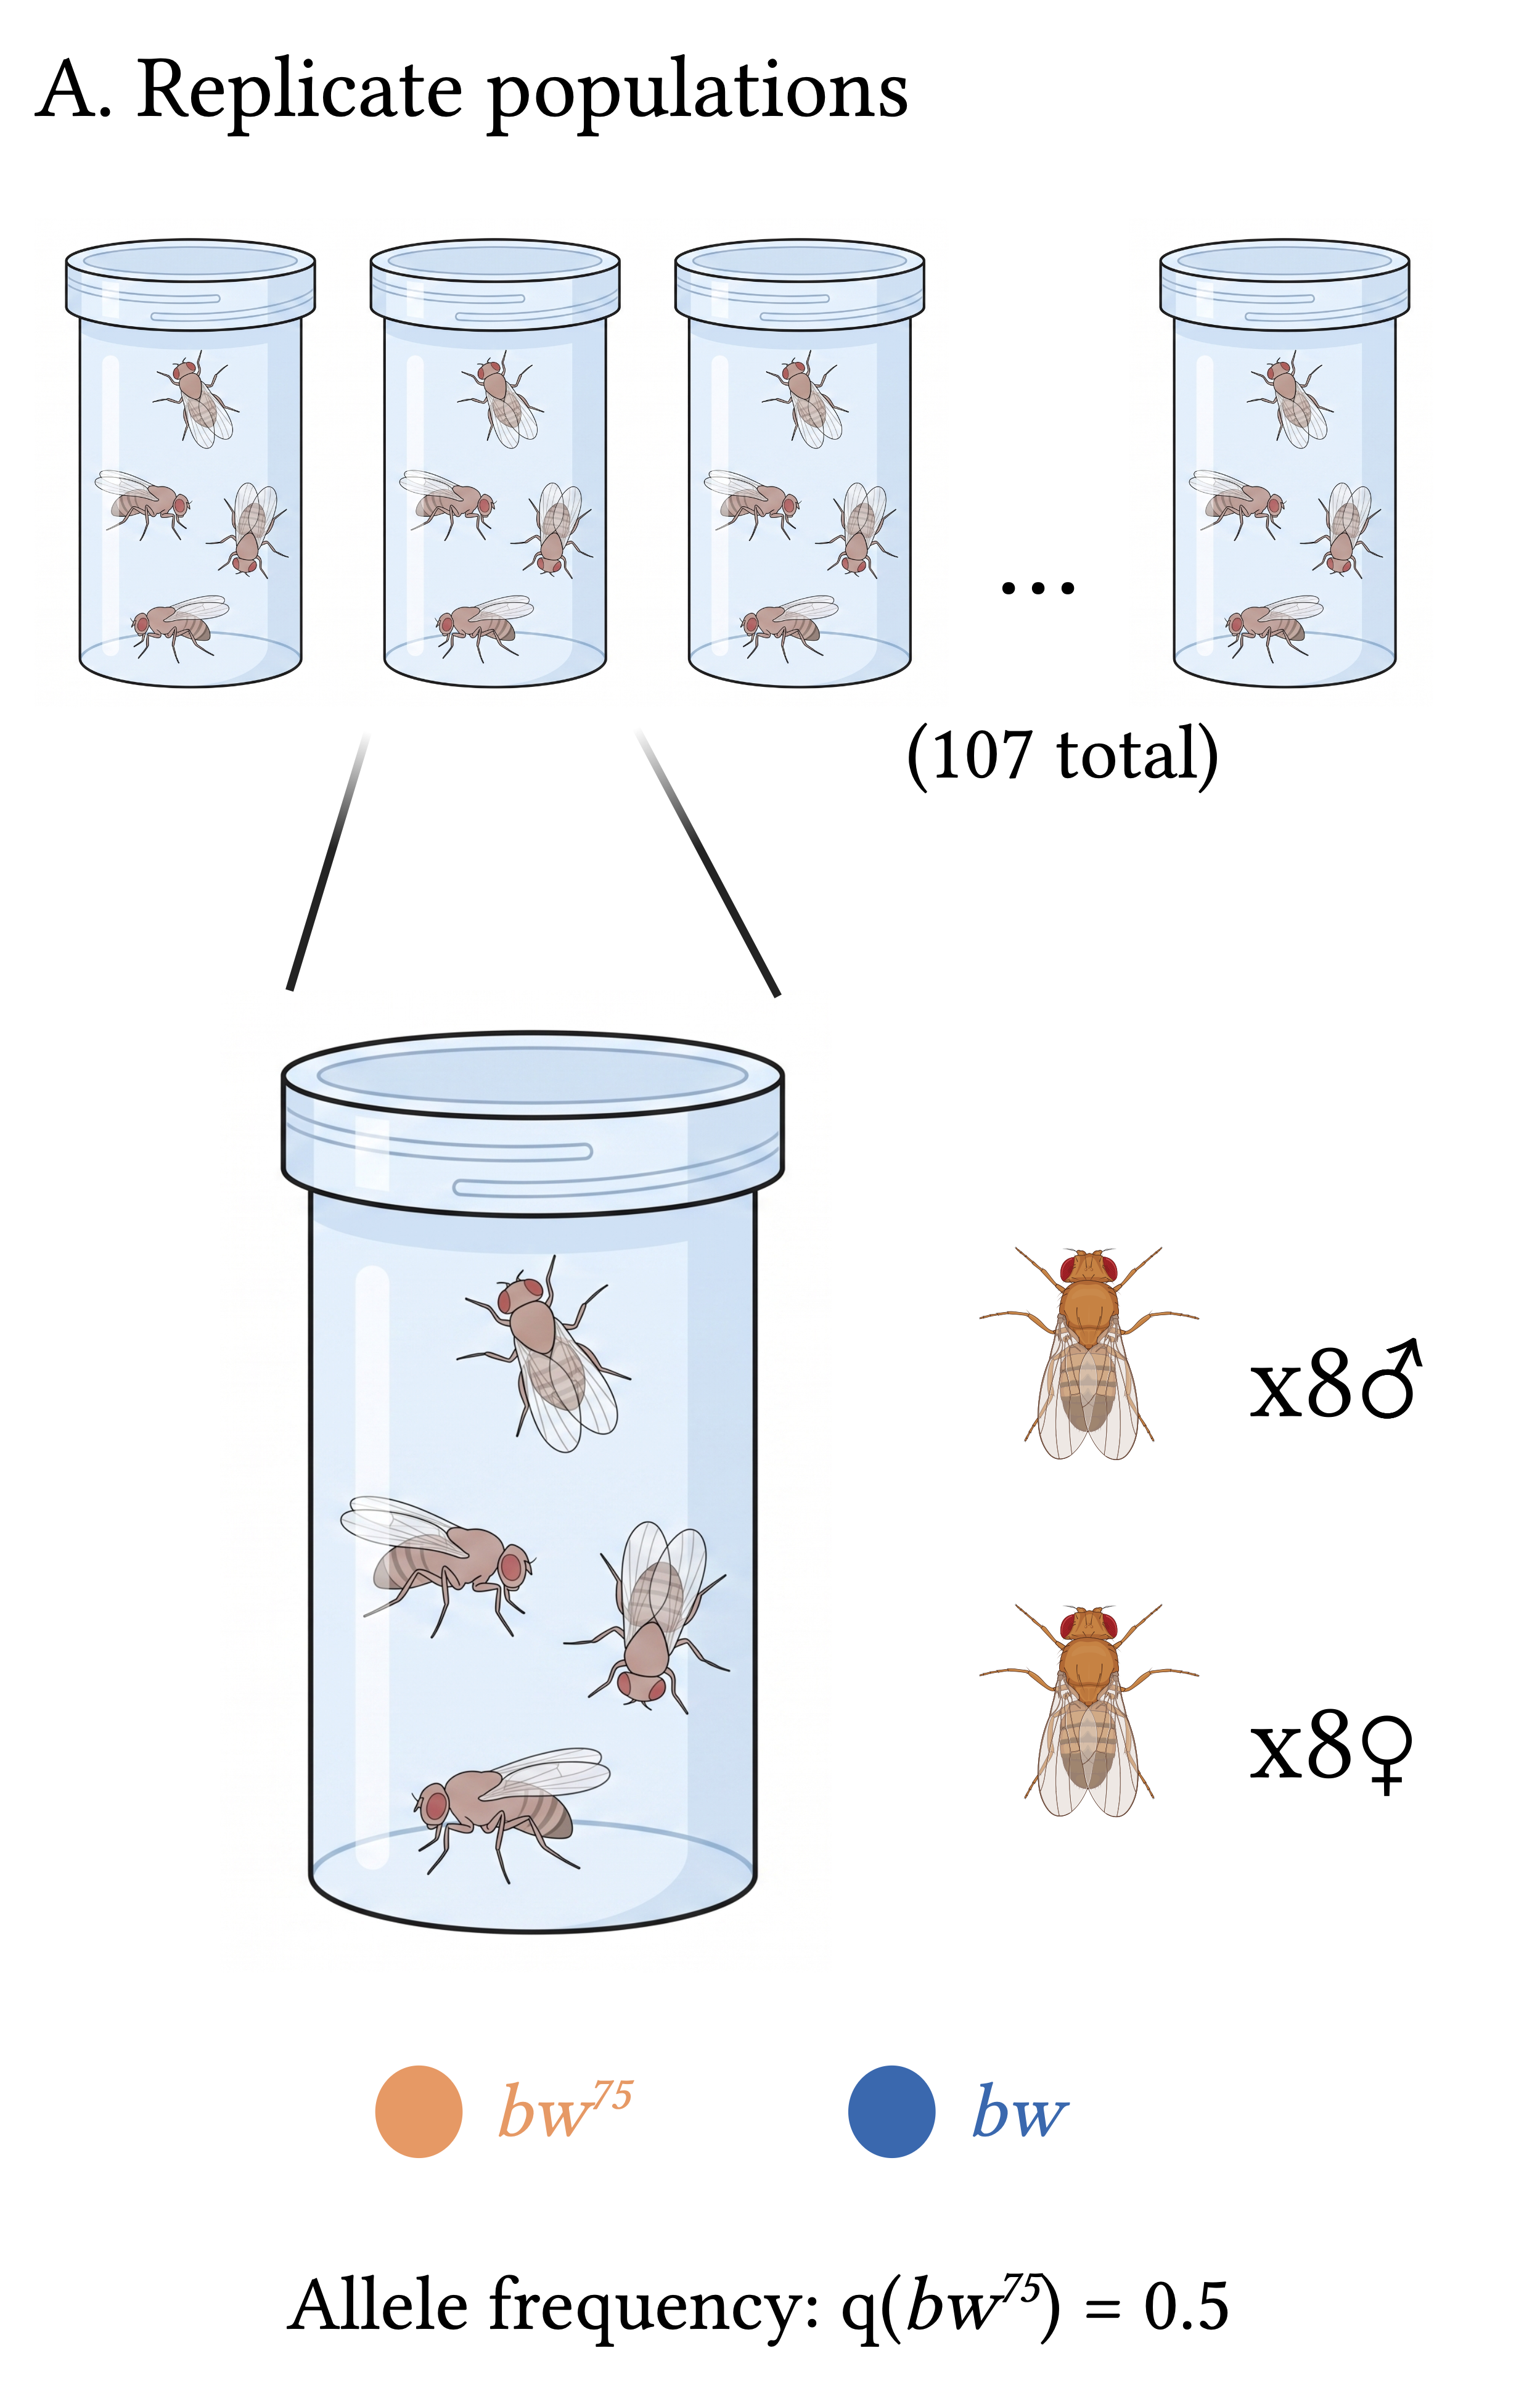
\includegraphics[width=\linewidth]{figures/buri-1.png}
    \end{minipage}
    \hfill
    \begin{minipage}[t]{0.34\textwidth}
        \vspace{0pt}
        \centering
        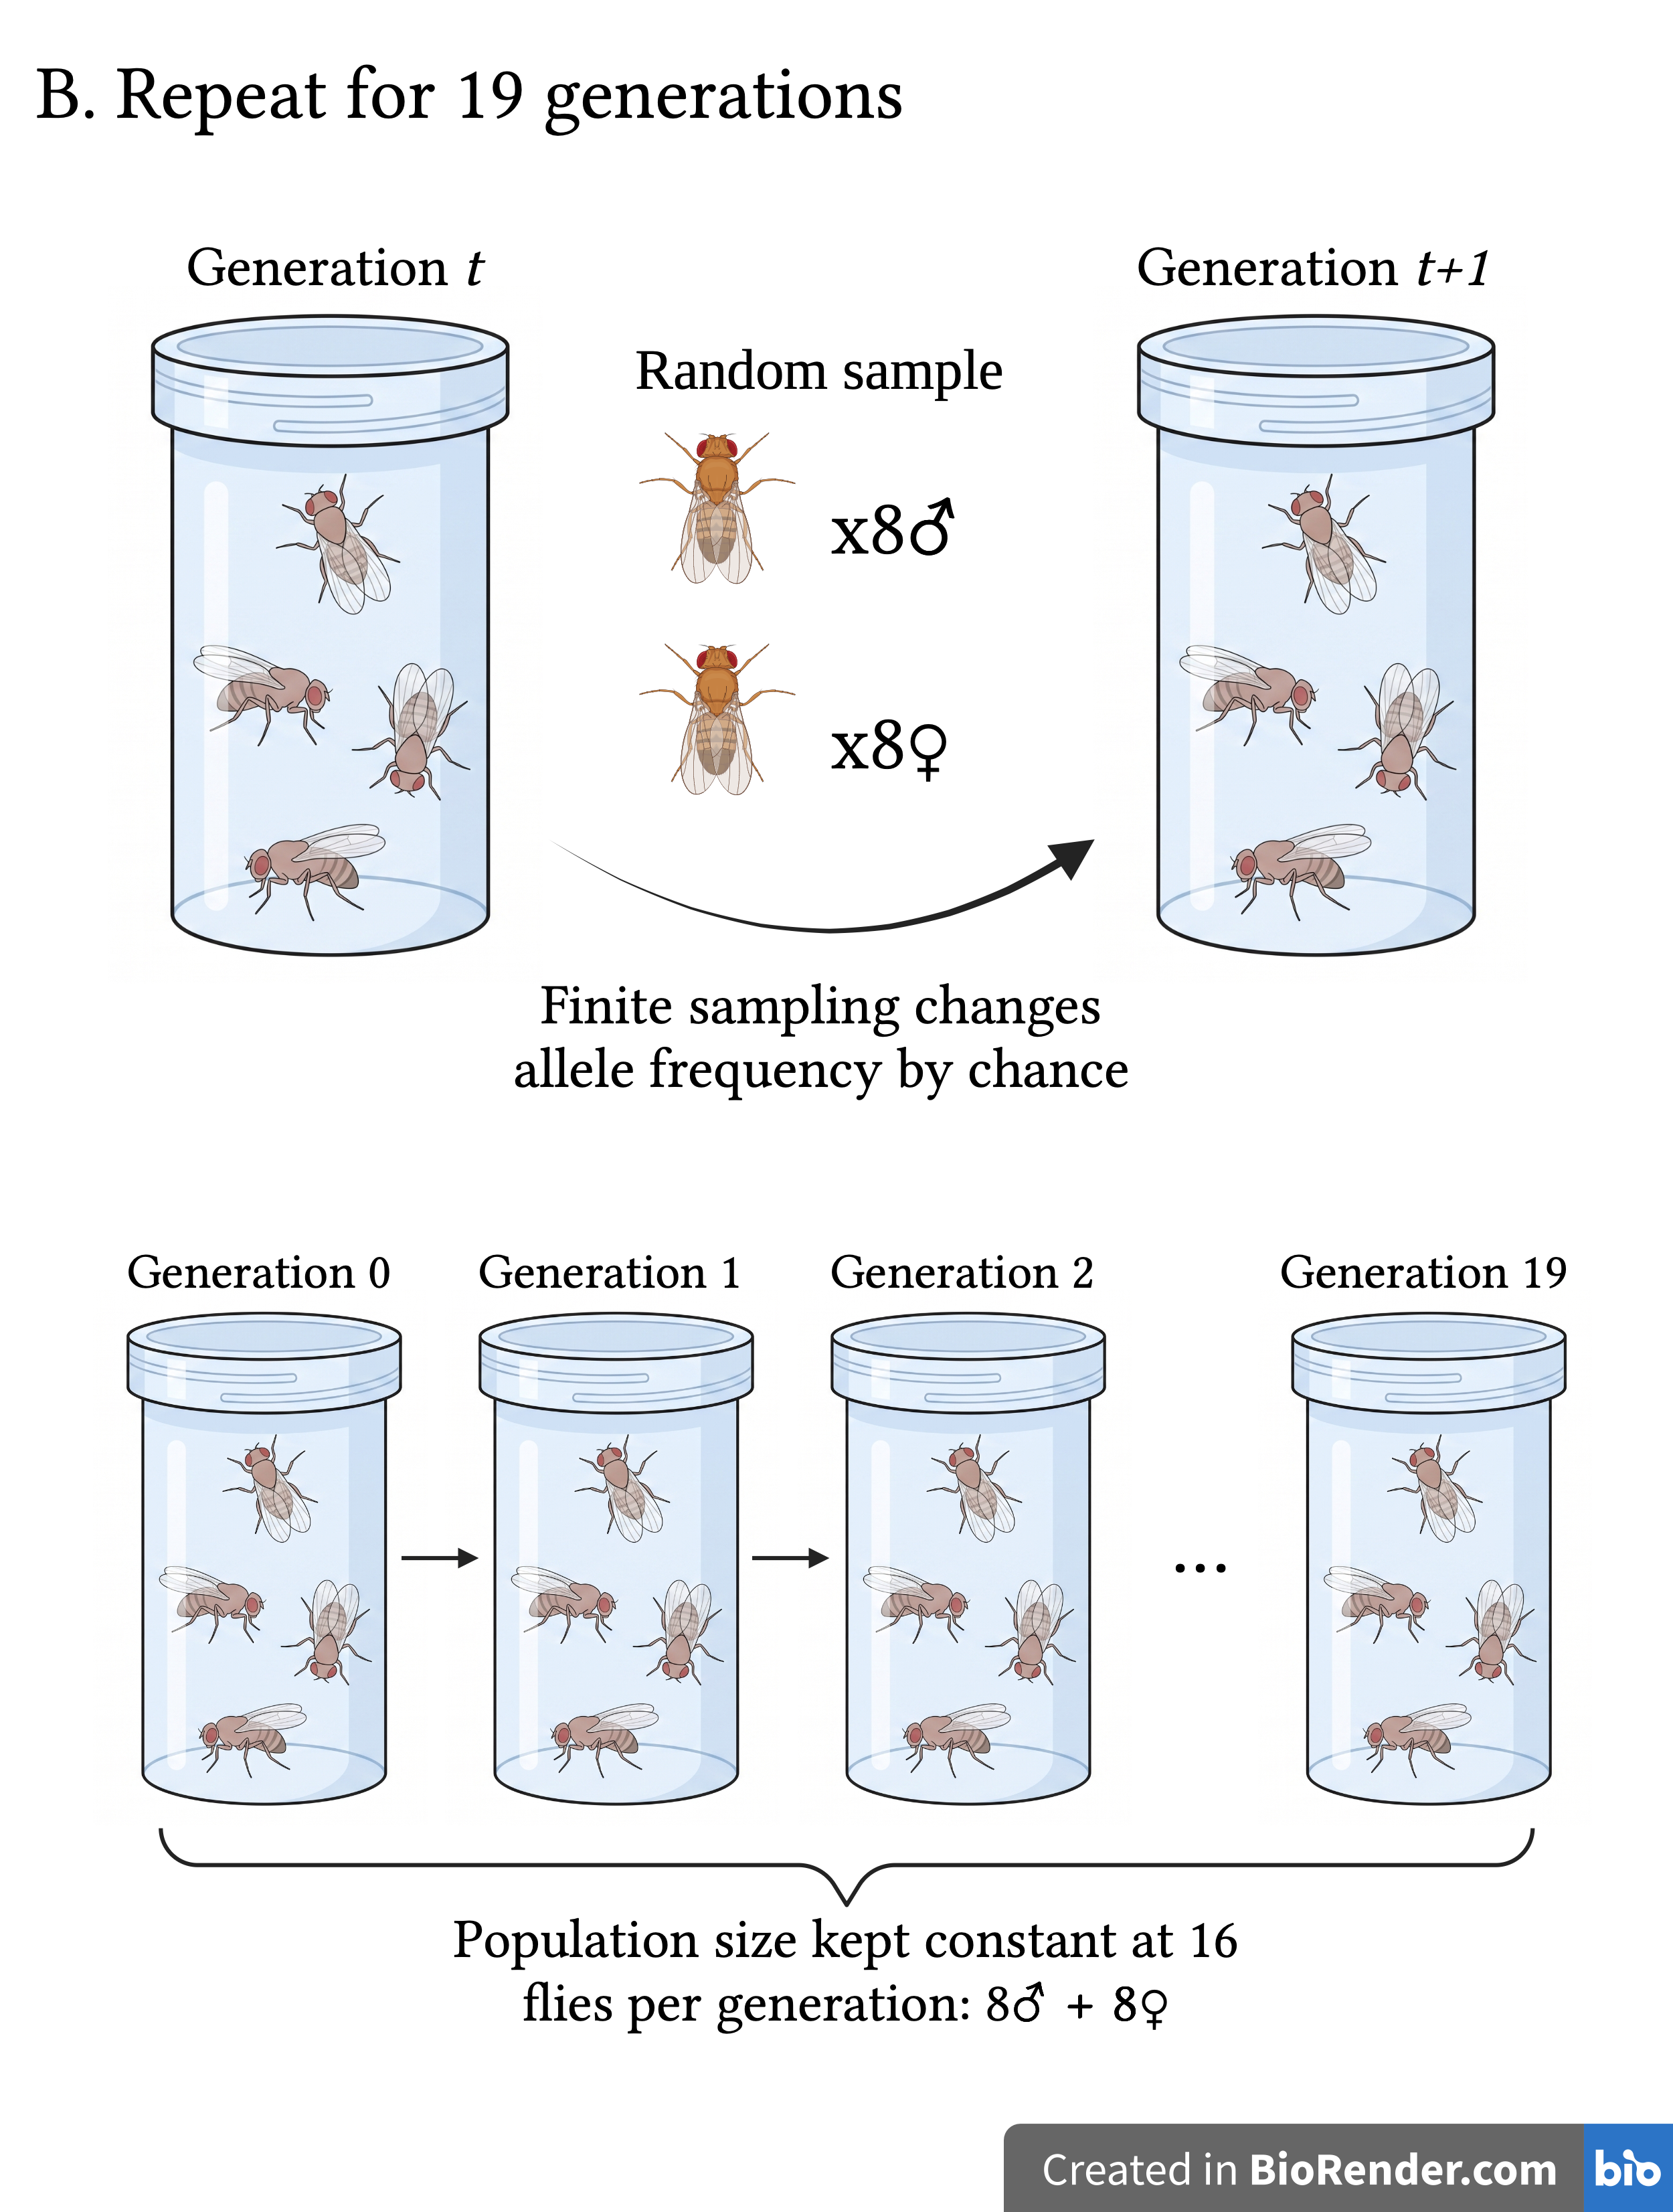
\includegraphics[width=\linewidth]{figures/buri-2.png}
    \end{minipage}
    \hfill
    \begin{minipage}[t]{0.31\textwidth}
        \vspace{0pt}
        \newcommand{\paneltitlefont}{\fontsize{6.75}{7}\selectfont}
\newcommand{\paneltextfont}{\fontsize{5}{4}\selectfont}
\newcommand{\panelcaptionfont}{\fontsize{5.5}{7}\selectfont}

\fontfamily{LinuxLibertineT-LF}\selectfont
\color{black!95}

\vspace{2mm}

{\paneltitlefont C. Replicates diverge\par}

\vspace{0.2em}

\noindent\makebox[\linewidth][c]{%
    \begin{minipage}{0.82\linewidth}
        \centering
        \paneltextfont
        Distribution of allele frequencies\\
        across replicate populations
    \end{minipage}%
}
\par

\vspace{0.1em}

\noindent\makebox[\linewidth][c]{%
    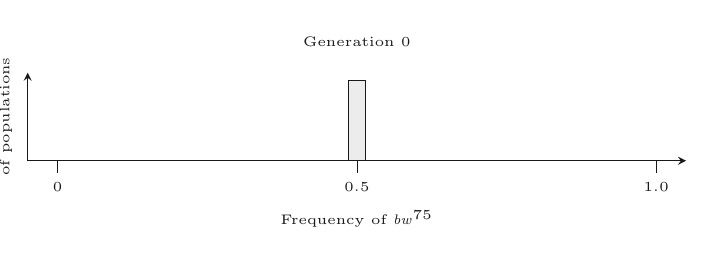
\begin{tikzpicture}[trim axis left,trim axis right]
    \begin{axis}[
        width=0.82\linewidth,
        height=2.7cm,
        title={Generation 0},
        title style={
            font=\paneltextfont,
            text=black!90
        },
        xmin=-0.05,
        xmax=1.05,
        ymin=0,
        ymax=1.1,
        xtick={0,0.5,1},
        xticklabels={$0$,$0.5$,$1.0$},
        ytick=\empty,
        xlabel={Frequency of \textit{bw}\textsuperscript{75}},
        ylabel={Relative number\\of populations},
        ylabel style={
            align=center,
            font=\paneltextfont,
            text=black!90
        },
        xlabel style={
            font=\paneltextfont,
            text=black!90
        },
        tick label style={
            font=\paneltextfont,
            text=black!90
        },
        axis lines=left,
        axis line style={
            draw=black!90,
            line width=0.3pt
        },
        tick style={
            draw=black!90,
            line width=0.25pt
        },
        font=\paneltextfont,
        ybar,
        bar width=6pt,
        enlarge x limits=false
    ]
        \addplot[
            fill=gray!15,
            draw=black!90,
            line width=0.3pt
        ]
        coordinates {
            (0.5,1)
        };
    \end{axis}
\end{tikzpicture}
}
\par

% \vspace{-1.1em}

\noindent\makebox[\linewidth][c]{%
    {\fontsize{7}{7}\selectfont\color{black!80}$\downarrow$}%
}
\par

% \vspace{-0.8em}

\noindent\makebox[\linewidth][c]{%
    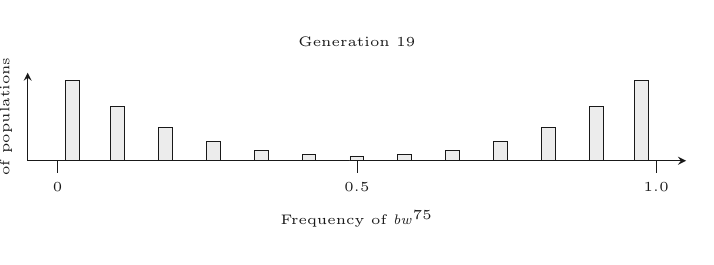
\begin{tikzpicture}[trim axis left,trim axis right]
    \begin{axis}[
        width=0.82\linewidth,
        height=2.7cm,
        title={Generation 19},
        title style={
            font=\paneltextfont,
            text=black!90
        },
        xmin=-0.05,
        xmax=1.05,
        ymin=0,
        ymax=1.1,
        xtick={0,0.5,1},
        xticklabels={$0$,$0.5$,$1.0$},
        ytick=\empty,
        xlabel={Frequency of \textit{bw}\textsuperscript{75}},
        ylabel={Relative number\\of populations},
        ylabel style={
            align=center,
            font=\paneltextfont,
            text=black!90
        },
        xlabel style={
            font=\paneltextfont,
            text=black!90
        },
        tick label style={
            font=\paneltextfont,
            text=black!90
        },
        axis lines=left,
        axis line style={
            draw=black!90,
            line width=0.3pt
        },
        tick style={
            draw=black!90,
            line width=0.25pt
        },
        font=\paneltextfont,
        ybar,
        bar width=5pt,
        enlarge x limits=false
    ]
        \addplot[
            fill=gray!15,
            draw=black!90,
            line width=0.3pt
        ]
        coordinates {
            (0.025,1.00)
            (0.10,0.68)
            (0.18,0.42)
            (0.26,0.24)
            (0.34,0.13)
            (0.42,0.08)
            (0.50,0.06)
            (0.58,0.08)
            (0.66,0.13)
            (0.74,0.24)
            (0.82,0.42)
            (0.90,0.68)
            (0.975,1.00)
        };
    \end{axis}
\end{tikzpicture}
}
\par

\vspace{0.6em}

\noindent\makebox[\linewidth][c]{%
    \begin{minipage}{0.82\linewidth}
        \centering
        \panelcaptionfont
        Genetic drift causes replicate populations to follow different paths even without selection.
    \end{minipage}
}
\par
    \end{minipage}

    \caption{The Buri experiment and genetic drift.
    Replicate populations were initialized with 16 heterozygous flies, giving an initial frequency of $q(bw^{75})=0.5$.
    The $bw^{75}$ allele frequency, denoted as $q(bw^{75})$ in (A), is written as $p_{\mathrm{red}}$ in the calculations above.
    Eight females and eight males were randomly selected to found each succeeding generation.
    Repeated sampling caused the allele-frequency distribution to spread toward loss and fixation.
    Panels A and B created with BioRender.com.
    Panel C is schematic and does not reproduce Buri's measured counts.}
    \label{fig:buri-drift}
\end{figure}